\documentclass[aspectratio=1610]{beamer}
\usepackage[utf8]{inputenc}
\usepackage{ragged2e}
\usepackage{xcolor}
\usepackage[italian]{babel}
\usetheme[progressbar=frametitle,titleformat=smallcaps]{metropolis}
\setbeamertemplate{frame numbering}[fraction]
\setbeamercovered{dynamic}
\definecolor{rosso}{RGB}{255, 0, 0}
\definecolor{giallo}{RGB}{254,212,23}
\hypersetup{colorlinks=true,linkcolor=black,urlcolor=rosso}
\setbeamercolor{palette primary}{fg=black, bg=giallo}
\setbeamercolor{background canvas}{bg=white}
\setbeamercolor{normal text}{fg=black}
\setbeamercolor{progress bar}{fg=rosso}
\setbeamercolor{framesubtitle}{fg=rosso}
\setbeamercolor{normal text .dimmed}{fg=giallo}
\setbeamercolor{block title alerted}{fg=rosso, bg=giallo}
\setbeamerfont{caption}{size=\tiny}
\setbeamerfont{caption name}{size=\tiny}
\setlength{\abovecaptionskip}{0pt}
\makeatletter
\metroset{block=fill}
\setlength{\metropolis@progressinheadfoot@linewidth}{1pt} 
\setlength{\metropolis@progressonsectionpage@linewidth}{1pt}
\setlength{\metropolis@titleseparator@linewidth}{1pt}
\makeatother

\title{DISPOSITIVI E TOPOLOGIE DI RETE}
\subtitle{componenti hardware e modelli geometrici di connettività}
\date{}
\institute{\textit{
        Fonti:
        \begin{itemize}
            \item[-] \href{https://it.wikipedia.org/wiki/Rete_di_computer}{Wikipedia}
            \item[-] \href{https://www.fastweb.it/fastweb-plus/digital-magazine/}{Fastweb Plus}
        \end{itemize}
    }
}

\begin{document}

\begin{frame}[plain, noframenumbering]
    \titlepage
\end{frame}

\section{DISPOSITIVI DI RETE}

\begin{frame}{DISPOSITIVI DI RETE}
    \begin{columns}
        \column{.5\textwidth}
            \justifying
            \begin{alertblock}{MODEM}
                \begin{minipage}{0.96\linewidth}
                    \justifying
                    Il Modem (modulator - demodulator) è un dispositivo di ricetrasmissione che ha 
                    funzionalità logiche di \textbf{modulazione/demodulazione} in trasmissioni analogiche e digitali. 
                    Si occupa di convertire (modula) i segnali digitali in impulsi analogici e, in fase di ricezione, 
                    riconverte (demodula) gli impulsi analogici in segnali digitali.\\
                    \bigskip
                    \tiny{\textbf{Curiosità}}\\
                    \tiny{\href{https://www.fastweb.it/fastweb-plus/digital-magazine/i-consigli-per-configurare-un-modem-router-wifi/}{Configurazione del Modem}}
                \end{minipage}
            \end{alertblock}
        \column{.5\textwidth}
            \begin{figure}
                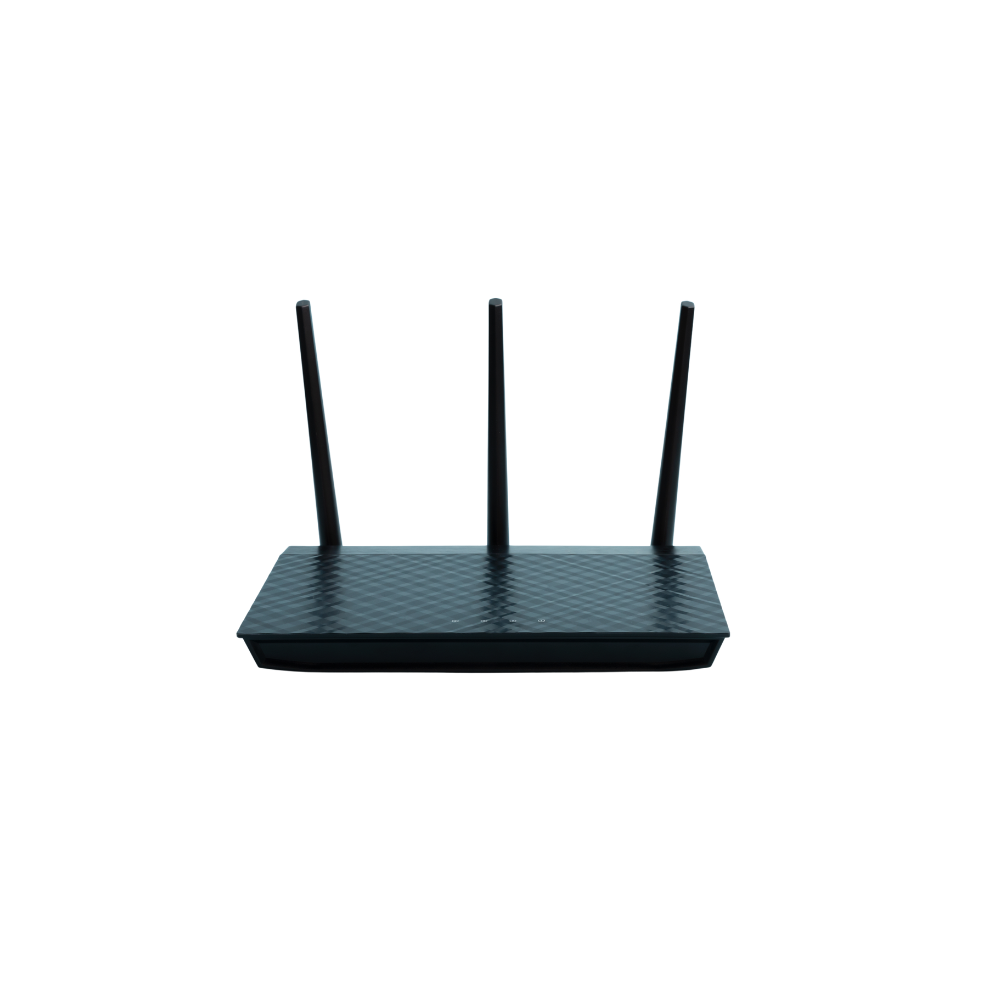
\includegraphics[width=\linewidth]{img/modemrouter.png}
                \caption{{Fonte \href{https://www.canva.com/}{Canva}}}
            \end{figure}
    \end{columns}
\end{frame}

\begin{frame}{DISPOSITIVI DI RETE}
    \begin{columns}
        \column{.5\textwidth}
            \justifying
            \begin{alertblock}{ROUTER}
                \begin{minipage}{0.96\linewidth}
                    \justifying
                    Un Router è un dispositivo che si occupa di \textbf{instradare i pacchetti} di dati attraverso la rete. 
                    Il router ha lo scopo di dirigere il traffico di tali pacchetti nel loro tragitto, 
                    sia che esso debba attraversare differenti reti locali private, o la rete Internet 
                    globale, fino a quando non raggiungono il nodo di destinazione.\\
                    \bigskip
                    \tiny{\textbf{Curiosità}}\\
                    \tiny{\href{https://www.fastweb.it/fastweb-plus/digital-magazine/come-trasformare-il-vecchio-router-in-un-access-point-wireless/}{Utilizzare il Router come Access Point (AP)}}
                \end{minipage}
            \end{alertblock}
        \column{.5\textwidth}
            \begin{figure}
                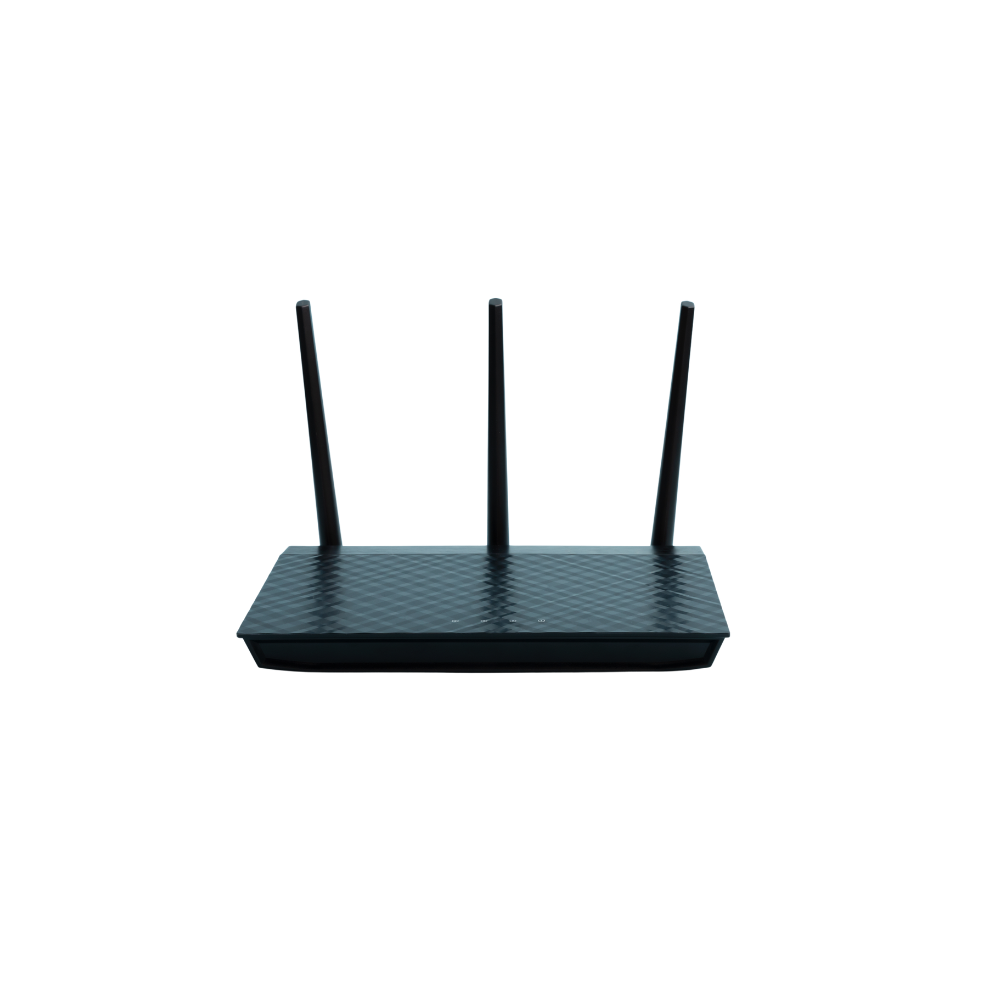
\includegraphics[width=\linewidth]{img/modemrouter.png}
                \caption{{Fonte \href{https://www.canva.com/}{Canva}}}
            \end{figure}
    \end{columns}
\end{frame}

\begin{frame}{DISPOSITIVI DI RETE}
    \begin{columns}
        \column{.5\textwidth}
            \justifying
            \begin{alertblock}{REPEATER}
                \begin{minipage}{0.96\linewidth}
                    \justifying
                    Un Repeater è un dispositivo elettronico che \textbf{riceve in ingresso un 
                    segnale e lo ritrasmette in uscita} (tipicamente con un segnale a potenza maggiore) 
                    cosicché la propagazione di questo può essere garantita anche a lunghe 
                    distanze senza eccessiva attenuazione e/o degradazione.
                \end{minipage}
            \end{alertblock}
        \column{.5\textwidth}
            \begin{figure}
                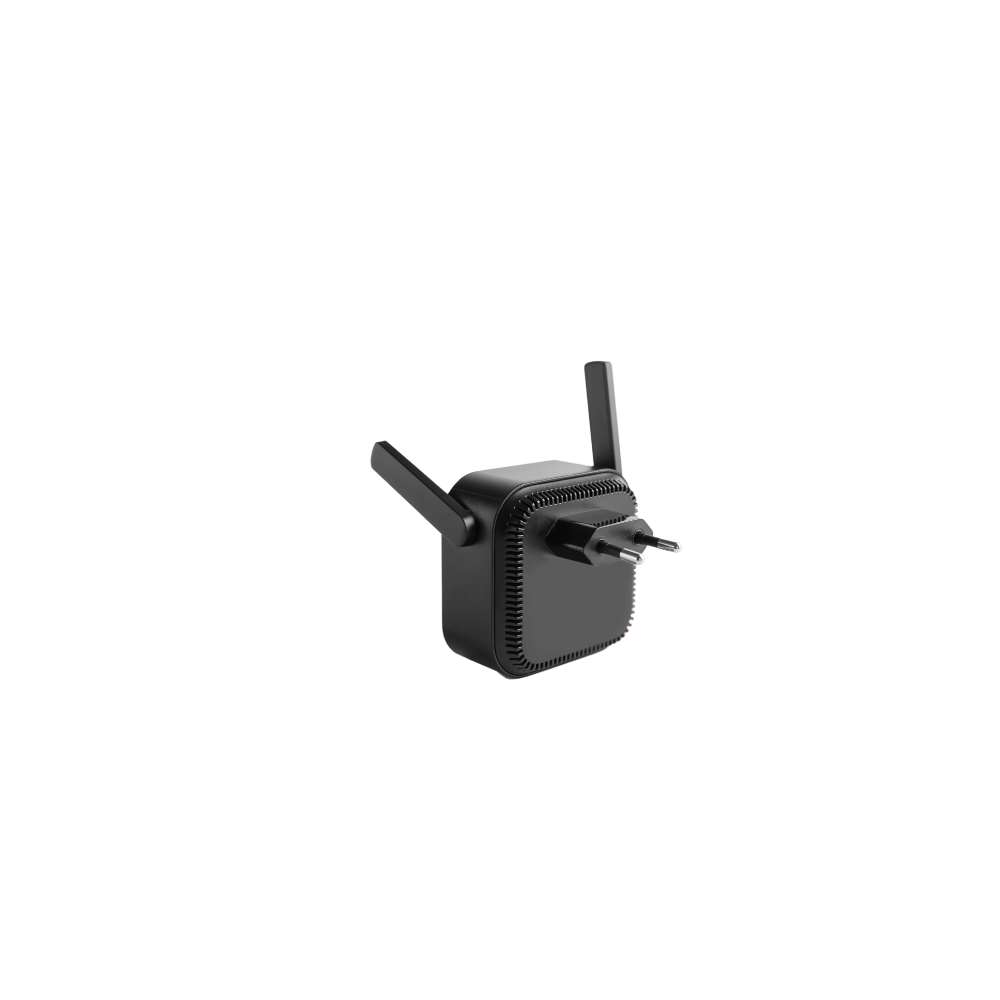
\includegraphics[width=\linewidth]{img/repeater.png}
                \caption{{Fonte \href{https://www.canva.com/}{Canva}}}
            \end{figure}
    \end{columns}
\end{frame}

\begin{frame}{DISPOSITIVI DI RETE}
    \begin{columns}
        \column{.5\textwidth}
            \justifying
            \begin{alertblock}{SWITCH}
                \begin{minipage}{0.96\linewidth}
                    \justifying
                    Uno Switch (commutatore) è un dispositivo che \textbf{collega insieme altri dispositivi}. 
                    Più cavi di rete sono collegati a uno switch per abilitare la comunicazione 
                    tra diversi dispositivi. Gli Switch gestiscono il flusso di dati attraverso 
                    una rete trasmettendo un pacchetto di rete ricevuto solo a uno o più 
                    dispositivi per i quali il pacchetto è destinato. I dispositivi che non sono in grado 
                    di instradare i dati verso il nodo corretto ma \textbf{effettuano trasmissioni broadcast}, 
                    vengono definiti \textbf{Hub}.\\
                    \bigskip
                    \tiny{\textbf{Curiosità}}\\
                    \tiny{\href{https://www.fastweb.it/fastweb-plus/digital-magazine/cos-e-un-bridge-di-rete-e-come-crearne-uno/}{Creare un Bridge di rete}}
                \end{minipage}
            \end{alertblock}
        \column{.5\textwidth}
            \begin{figure}
                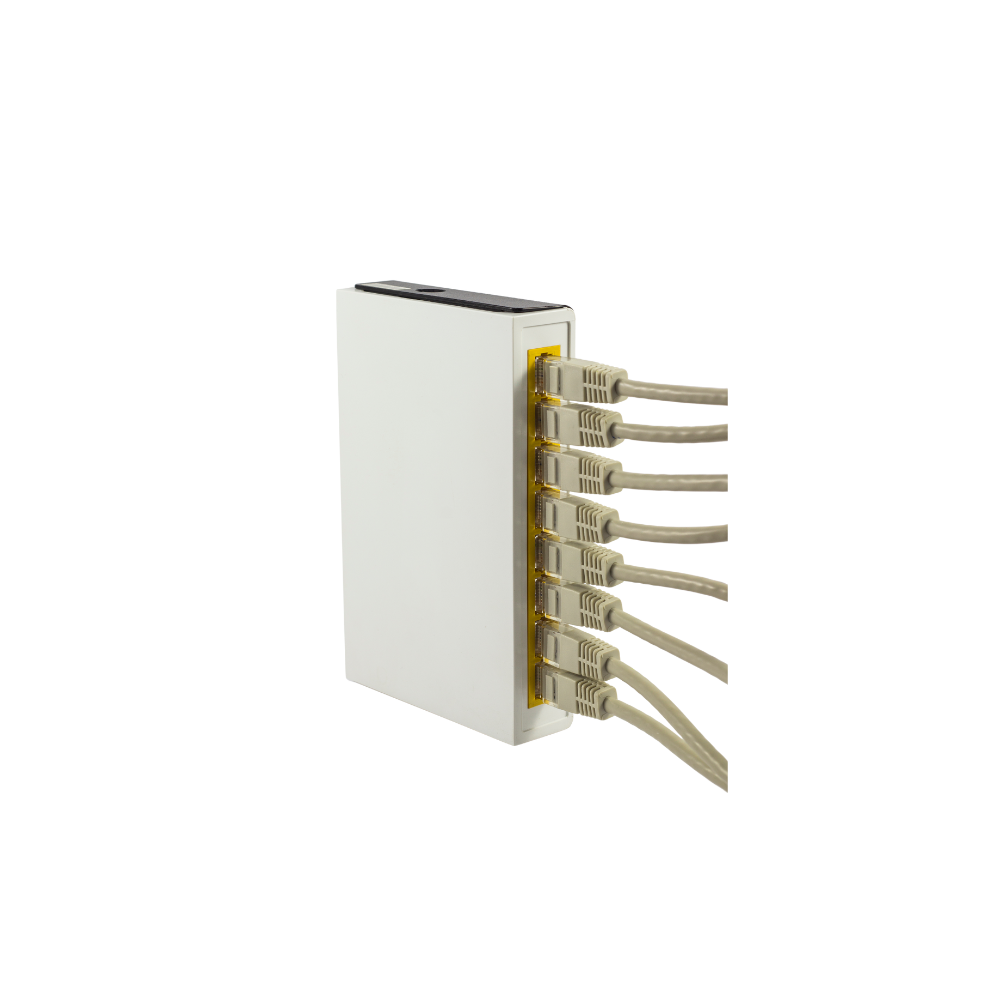
\includegraphics[width=\linewidth]{img/hubbridgeswitch.png}
                \caption{{Fonte \href{https://www.canva.com/}{Canva}}}
            \end{figure}
    \end{columns}
\end{frame}

\section{TOPOLOGIE DI RETE}

\begin{frame}{TOPOLOGIA DI RETE}
    \begin{alertblock}{DEFINIZIONE}
        \begin{minipage}{0.98\linewidth}
            \justifying
            La topologia di rete è il \textbf{modello geometrico} (grafo) finalizzato a \textbf{rappresentare 
            le relazioni di connettività}, fisica o logica, tra gli elementi costituenti la rete 
            stessa (nodi). Gli elementi fondamentali della topologia sono \textbf{i nodi e gli archi} (link). 
            Il nodo individua un elemento della rete connotato da specifiche funzionalità, 
            mentre l'arco evidenzia la relazione di connettività tra i nodi.
        \end{minipage}
    \end{alertblock}
\end{frame}

\begin{frame}{TOPOLOGIE DI RETE}
    \begin{columns}
        \column{.5\textwidth}
            \justifying
            \begin{alertblock}{STELLA}
                \begin{minipage}{0.96\linewidth}
                    \justifying
                    \textbf{PRO}
                    \begin{itemize}
                        \item Facilità di gestione e configurazione
                        \pause
                        \item Isolamento dei guasti
                        \pause
                        \item Scalabilità semplice
                    \end{itemize}
                    \pause
                    \textbf{CONTRO}
                    \begin{itemize}
                        \item Dipendenza dal nodo centrale
                        \pause
                        \item Possibilità di costi elevati
                        \pause
                        \item Possibile \href{https://it.wikipedia.org/wiki/Collo\_di\_bottiglia\_(ingegneria)}{Collo di bottiglia}
                    \end{itemize}
                \end{minipage}
            \end{alertblock}
        \column{.5\textwidth}
            \begin{figure}
                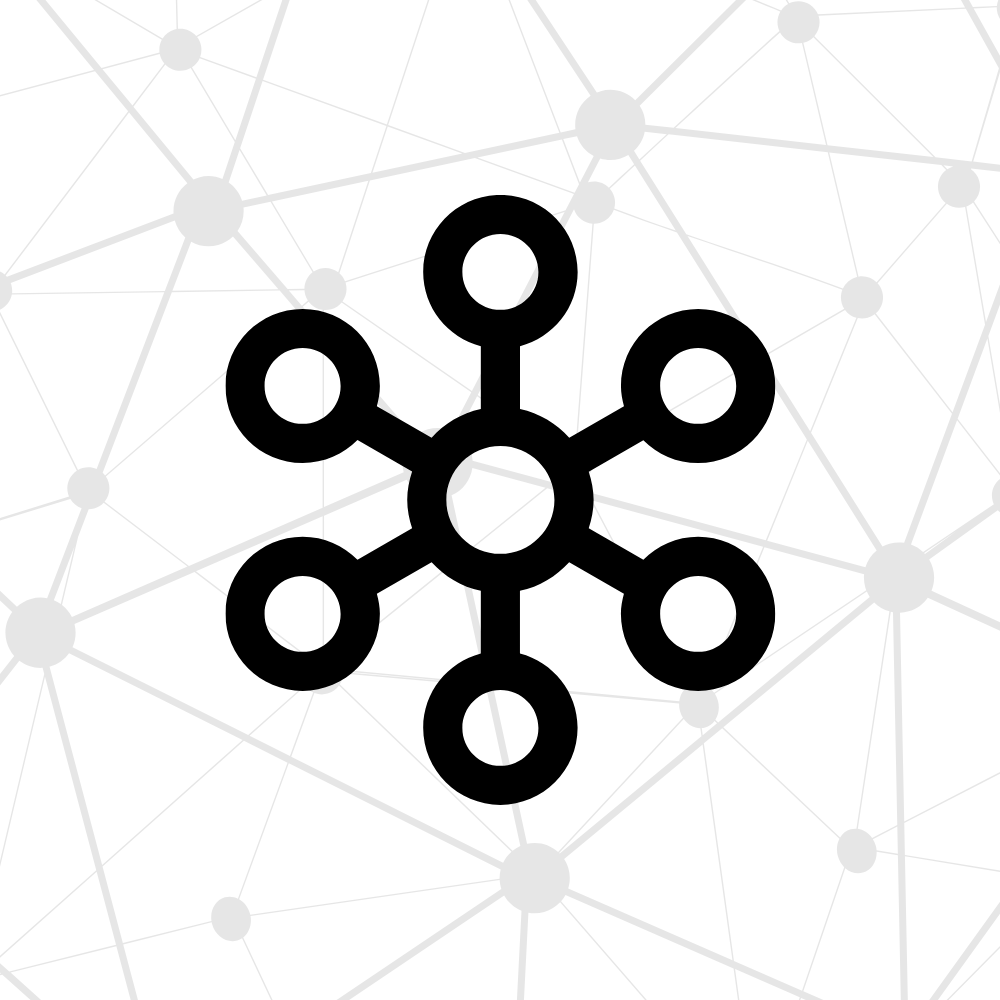
\includegraphics[width=\linewidth]{img/stella.png}
                \caption{{creata con \href{https://www.canva.com/}{Canva}}}
            \end{figure}
    \end{columns}
\end{frame}

\begin{frame}{TOPOLOGIE DI RETE}
    \begin{columns}
        \column{.5\textwidth}
            \justifying
            \begin{alertblock}{ANELLO}
                \begin{minipage}{0.96\linewidth}
                    \justifying
                    \textbf{PRO}
                    \begin{itemize}
                        \item Non necessitano di un nodo centrale
                        \pause
                        \item Banda uniforme (oraria/antioraria)
                        \pause
                        \item Tolleranza ai guasti
                    \end{itemize}
                    \pause
                    \textbf{CONTRO}
                    \begin{itemize}
                        \item Difficoltà nella scalabilità
                        \pause
                        \item Costi di sincronizzazione e gestione
                        \pause
                        \item Limiti al numero di nodi
                    \end{itemize}
                \end{minipage}
            \end{alertblock}
        \column{.5\textwidth}
            \begin{figure}
                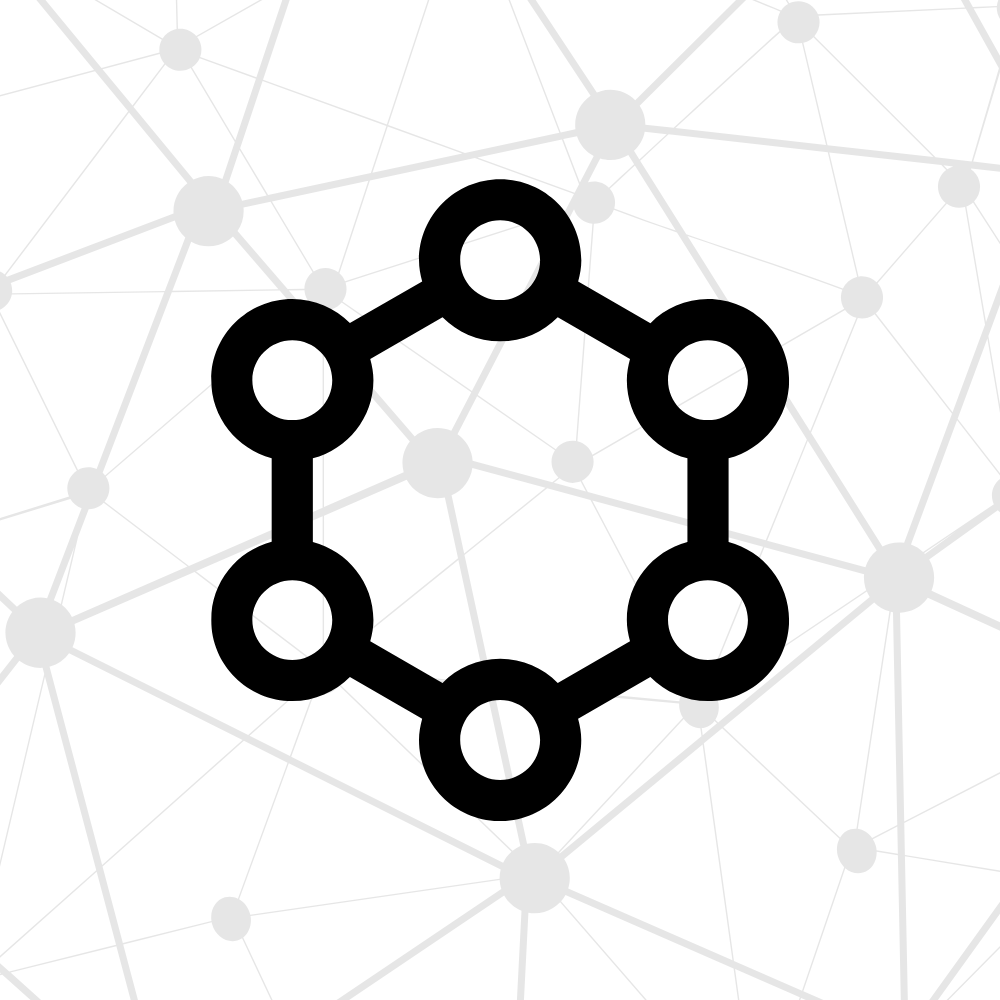
\includegraphics[width=\linewidth]{img/anello.png}
                \caption{{creata con \href{https://www.canva.com/}{Canva}}}
            \end{figure}
    \end{columns}
\end{frame}

\begin{frame}{TOPOLOGIE DI RETE}
    \begin{columns}
        \column{.5\textwidth}
            \justifying
            \begin{alertblock}{BUS}
                \begin{minipage}{0.96\linewidth}
                    \justifying
                    \textbf{PRO}
                    \begin{itemize}
                        \item Semplicità
                        \pause
                        \item Economicità per reti ristrette
                        \pause
                        \item Scalabilità semplice
                    \end{itemize}
                    \pause
                    \textbf{CONTRO}
                    \begin{itemize}
                        \item Single Point Of Failure (\href{https://it.wikipedia.org/wiki/Single_point_of_failure}{SPOF})
                        \pause
                        \item Difficoltà della gestione delle connessioni
                        \pause
                        \item Prestazioni scadenti con carichi elevati
                    \end{itemize}
                    \tiny{\textbf{Curiosità}}\\
                    \tiny{\href{https://www.fastweb.it/fastweb-plus/digital-magazine/congestione-della-rete-cosa-fare/}{Congestione della rete}}
                \end{minipage}
            \end{alertblock}
        \column{.5\textwidth}
            \begin{figure}
                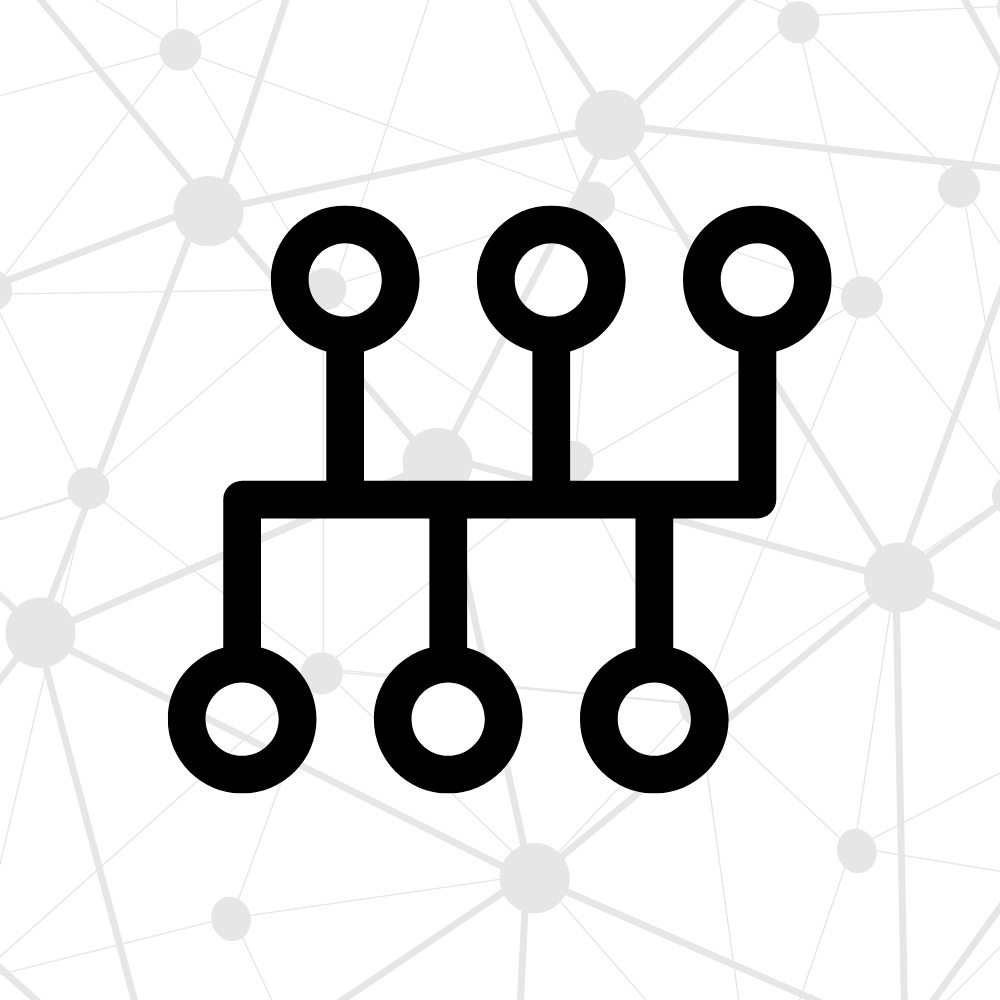
\includegraphics[width=\linewidth]{img/bus.png}
                \caption{{creata con \href{https://www.canva.com/}{Canva}}}
            \end{figure}
    \end{columns}
\end{frame}

\begin{frame}{TOPOLOGIE DI RETE}
    \begin{columns}
        \column{.5\textwidth}
            \justifying
            \begin{alertblock}{MAGLIA}
                \begin{minipage}{0.96\linewidth}
                    \justifying
                    \textbf{PRO}
                    \begin{itemize}
                        \item Robustezza ai guasti
                        \pause
                        \item Alta affidabilità
                        \pause
                        \item Prestazioni elevate
                    \end{itemize}
                    \pause
                    \textbf{CONTRO}
                    \begin{itemize}
                        \item Costi di creazione e gestione elevati
                        \pause
                        \item Configurazione complessa
                        \pause
                        \item Possibilità di eccessiva ridondanza
                    \end{itemize}
                \end{minipage}
            \end{alertblock}
        \column{.5\textwidth}
            \begin{figure}
                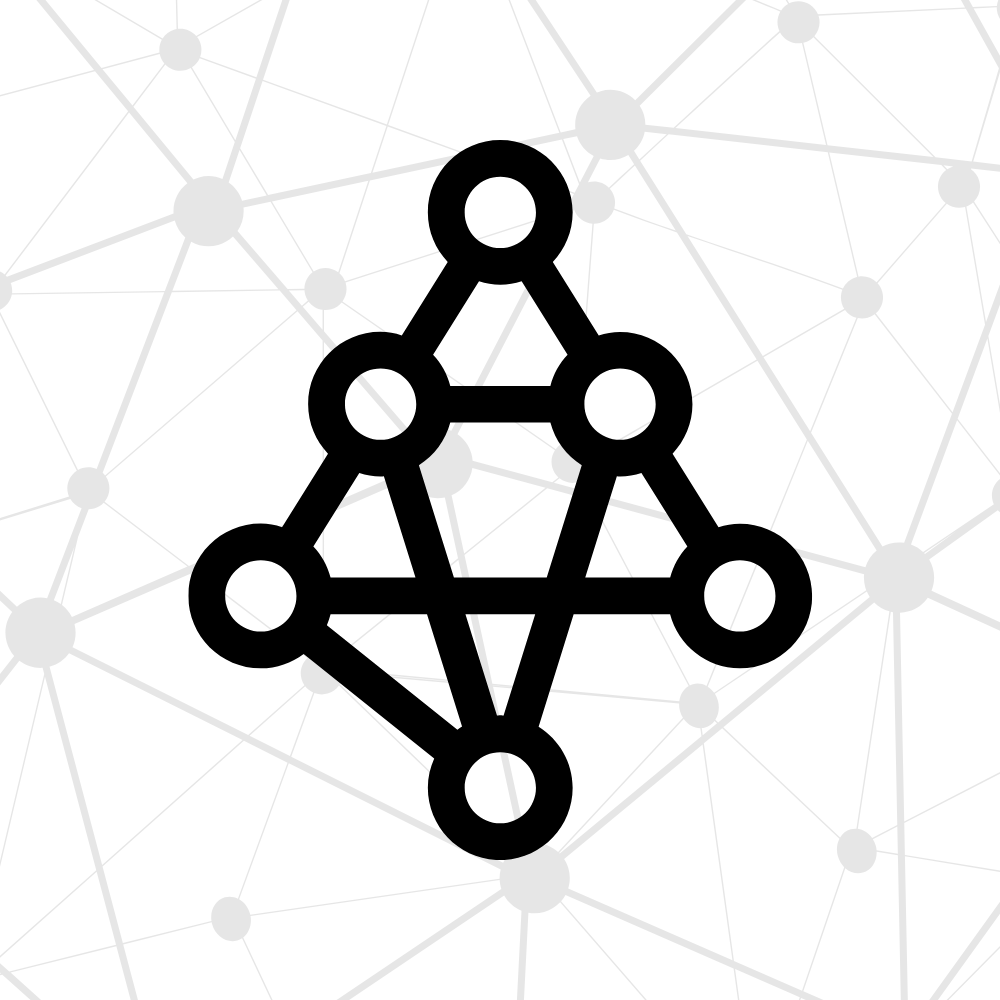
\includegraphics[width=\linewidth]{img/maglia.png}
                \caption{{creata con \href{https://www.canva.com/}{Canva}}}
            \end{figure}
    \end{columns}
\end{frame}

\end{document}